\documentclass{article}

% Language setting
% Replace `english' with e.g. `spanish' to change the document language
\usepackage[english]{babel}

% Set page size and margins
% Replace `letterpaper' with `a4paper' for UK/EU standard size
\usepackage[a4paper,top=2cm,bottom=2cm,left=3cm,right=3cm,marginparwidth=1.75cm]{geometry}

% Useful packages
\usepackage{amsmath}
\usepackage{graphicx}
\usepackage[colorlinks=true, allcolors=blue]{hyperref}
\usepackage{xcolor}
\usepackage{listings}

\colorlet{mygray}{black!30}
\colorlet{mygreen}{green!60!blue}
\colorlet{mymauve}{red!60!blue}

\lstset{
  backgroundcolor=\color{gray!10},  
  basicstyle=\ttfamily,
  columns=fullflexible,
  breakatwhitespace=false,      
  breaklines=true,                
  captionpos=b,                    
  commentstyle=\color{mygreen}, 
  extendedchars=true,              
  frame=single,                   
  keepspaces=true,             
  keywordstyle=\color{blue},      
  language=c++,                 
  numbers=none,                
  numbersep=5pt,                   
  numberstyle=\tiny\color{blue}, 
  rulecolor=\color{mygray},        
  showspaces=false,               
  showtabs=false,                 
  stepnumber=5,                  
  stringstyle=\color{mymauve},    
  tabsize=3,                                     
  title=\lstname 
}


\lstnewenvironment{code}[2][]{%
  \lstset{%
    numbers = left,
    title   = #2,
    #1,
  }%
}{}

\title{Homework 3}
\author{Steinarr Hrafn Höskuldsson}

\newcommand{\mycomment}[1]{}
\usepackage{fancyhdr}
\fancypagestyle{firststyle}
{
   \fancyhf{}
   \fancyhead[L]{Mechatronics 2}
   
   \renewcommand{\headrulewidth}{0pt} % removes horizontal header line
}
\setlength{\parskip}{1em}

\setlength{\parindent}{0pt}
\begin{document}

\mycomment{

\begin{figure}[h]
    \centering
    \includegraphics[width=0.75\textwidth]{LAB3/Basic1.png}
    \caption{"Switch test" Breadboard set up}
    \label{fig:Switch_test}
\end{figure}

\lstinputlisting[caption=Defining 'ColorMatch' state, label={lst:colormatch}, language=Python, firstline=44, lastline=52]{LAB3/Basic.py}

} % end of comment

\pagestyle{firststyle}
{\let\newpage\relax\maketitle}
\section*{What is an 8-bit processor?}
The '8-bit' part of an 8-bit processor refers to the size of each operating register. The processor works with 8 bit numbers at a time.

\section*{How does a Microcontroller work?}
A microcontroller fetches one instruction at a time from a memory that holds the program instructions, typically a ROM or Flash memory. The microcontroller then executes that instruction. An instruction might for example be to copy a value from one part of memory to another. This cycle of fetching and executing instructions is driven by the clock signal. The data that the microcontroller interacts with is stored on the RAM (Random Access Memory). Most of the RAM can only hold data however part of the RAM contains the working registers which are different in that the microprocessor can do work on them.

The microprocessor will store a Program Counter, the location of the next instruction to fetch, in its working registers and an instruction will include proper increments to the Program Counter.

A subroutine is programmed by changing the Program Counter to a completely different part of the program. Subroutines must then start by storing the previous Program counter somewhere on the RAM and perhaps other registers as well. After executing, the subroutine should then restore the Program Counter and other registers to the stored values before jumping back to the proper spot in the program (as defined by the stored Program Counter value)

Keep track of where to store things on the RAM the microprocessor has a Stack Pointer to the next free memory space in RAM and that value gets incremented or decremented as memory is used or freed.

A microprocessor typically has some peripherals such as but not limited to I/O (input and outputs), ADC (Analog to Digital Converter), UART (Universal Asynchronous Reciever Transmitter) and Timers. Often a peripheral is able to set a flag when something interesting has happened. 

To increase programming efficiency a microprocessor usually has Interrupts, the ability to halt program execution and run a subroutine when such a flag gets set. The The interrupt routines are defined in a special Interrupt Table and interrupts must be enabled by setting the proper flag in the Status register. Typically the interrupt subroutine will disable interrupts while running and then restore them once done. And since interrupts might for example happen in the middle of some calculations an interrupt routine will store the state of the Status register on the RAM in order to restore it to how it was before returning.

\newpage
\section*{Library for controlling an LED}
The augmented bitwise operators \verb"|=, &= and ^=" can be used to change only one bit of a number.

In the following code files they have been implemented to turn on, off, or toggle, the onboard LED of an Arduino.

\lstinputlisting[caption=LEDlib.h]{HW3/LEDlib.h}
\lstinputlisting[caption=LEDlib.c]{HW3/LEDlib.c}
\lstinputlisting[caption=main.c]{HW3/main.c}


\section*{Final Project - AirDrums}
Last week I sourced an Accelerometer from Hannes, wired it to an Arduino and read and printed the analog value from it using the Arduino IDE environment and examined the analog values on an interactive plot.

Next week I plan on testing out a few different methods of mounting the sensor and what affect those will have on the response to a thigh clap.

If I don't get lost in testing different mounting methods I will start testing out methods to filter and detect thigh claps.

Figure \ref{hw3:fig:software} shows a rough outline of the software, I envision a master loop style program. The biggest challenge will probably be to implement the filter and detection algorithm since it will have to keep track of multiple signals at a time and probably look at how they behave over time.


\begin{figure}[h]
    \centering
    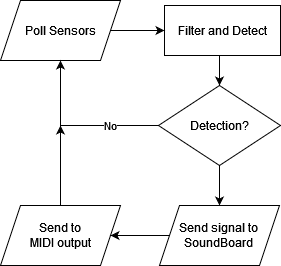
\includegraphics[width=0.5\textwidth]{HW3/softwareblock.png}
    \caption{Final project - software block diagram}
    \label{hw3:fig:software}
\end{figure}

\end{document}

